\graphicspath{{chapters/05/images/}}
\chapter{Expression analysis}

\section{Introduction}

	\subsection{Expressed genes}
	The expressed genes are those genes that have been transcribed.
	A gene expression profile of a cell is the snapshot of which genes are expressed in that cell at the time the sample was taken.
	Knowing which genes are expressed in a cell allows the identification of new genes or transcripts and the comparison of expression profiles between samples.
	Variability in gene expression is mainly due to alternative splicing and different regulation.
	It can be analyzed to uncover characteristics of diseases, development and dynamic responses to stimuli.

	\subsection{Differential gene expression (DGE)}
	Gene expression profiles are extremely heterogeneous, since they vary based on the individual, tissue, condition and cells of origin.
	Variability is mainly due to alternative splicing and different regulation.
	During a differential gene expression experiment the expression profile of genes is compared between samples.
	Comparison can be done between:

	\begin{multicols}{2}
		\begin{itemize}
			\item Different cells.
			\item Different tissues.
			\item Different disease states.
			\item Different developmental stages.
			\item Different culture conditions.
		\end{itemize}
	\end{multicols}
	For example, a basic experiment can be done by simply measuring two expression profiles, subtract the overlap, obtain the difference and interpret it.
	Two things to pay attention to are negative and positive controls and the range of variability within samples.

		\subsubsection{Differential gene expression workflow}
		A typical differential gene expression analysis workflow consists of:

		\begin{multicols}{2}
			\begin{enumerate}
				\item Formulation of the biological question.
				\item Experimental design: choice of platform, control and replicates to have trustful data.
				\item Running the experiment.
				\item Image processing done by a machine.
				\item Low-level analysis: data pre-processing with normalization.
				\item High-level analysis: actual data analysis.
				\item Obtaining biological conclusions and interpretation of results.
			\end{enumerate}
		\end{multicols}

		\subsubsection{High throughput methods}
		To perform differential gene expression analysis high throughput methods can be used.
		Their pros and cons are described in table \ref{tab:high-through-dge}.

		\begin{table}[H]
			\centering
			\begin{tabular}{|c|c|}
				\hline
				Pros & Cons\\
				\hline
				Fast & Difficult to filter non coding RNA\\
				Comprehensive (entire genomes) & Not enough attention to design\\
				Easy & Artefacts\\
				Getting cheaper & Cannot afford controls or replicates\\
				\hline
			\end{tabular}
			\caption{High throughput methods pros and cons}
			\label{tab:high-through-dge}
		\end{table}

		Even if the cons of high-throughput methods are important obstacles for performing complete, trustful analysis, these methods are becoming always better (less errors), cheaper and the computational side of the experiment is also improving to make the best out of the output data.

	\subsection{Main technologies}

	\begin{multicols}{2}
		\begin{itemize}
			\item Microarray technology: used more in the past.
			\item RNA-seq technology: today's best approach to DGE analysis, as it is becoming more accessible and allows for transcriptome sequencing and quantification of mRNA transcripts.
		\end{itemize}
	\end{multicols}

	\subsection{Databases}
	Repositories of array and NGS data mainly contain expression data.
	All of these databases can be interrogated with Bioconductor packages in R.

		\subsubsection{Gene expression omnibus}
		The gene expression omnibus or GEO is a public repository for the archiving and distribution of gene expression data submitted by the scientific community.
		It is a curated, online resource for gene expression data browsing, query, analysis and retrieval.
		It is convenient for the deposition of gene expression data as required by funding agencies and journals.
		Submitted data needs to include:

		\begin{multicols}{4}
			\begin{itemize}
				\item Platform.
				\item Sample.
				\item Series.
				\item Dataset.
			\end{itemize}
		\end{multicols}

		GEO is connected to repositories specifically tailored to store raw data like BioProject or SRA.

		\subsubsection{ArrayExpress}
		ArrayExpress or EBI si another online repository of array expression data.

		\subsubsection{Gene expression Atlas}
		The gene expression atlas GXE NCBI provides information on gene expression patterns.
		The raw data is re-analysed with common pipelines.




\section{Microarrays}

	\subsection{Introduction}
	Microarrays have been introduced at the beginning of the $2000$s and were the first high throughput technology.
	They are useful to investigate a variety of omics data, for example:

	\begin{multicols}{2}
		\begin{itemize}
			\item Genomic and transcriptomic profiles.
			\item The methylome.
			\item DNA-protein interactions.
			\item The microbiome.
		\end{itemize}
	\end{multicols}

	Data interpretation is subject to specific computational analyses.
	Microarrays are considered high-throughput because they monitor thousands of genes in parallel.
	Each spot contains multiple and identical DNA probes and thousands of spots are disposed as a matrix on a solid support, the microarray.
	Microarrays are basically a glass surface hosting spots containing redundant information about the DNA.

	\subsection{Fabrication}
	Microarrays can be fabricated using different technologies.
	Probes can be:

	\begin{multicols}{3}
		\begin{itemize}
			\item Oligonucleotides.
			\item cDNA.
			\item Small PCR fragments related to specific mRNA.
		\end{itemize}
	\end{multicols}

	The probes are synthesized and placed on the support and can have different lengths, usually between $25$ and $60nt$, to ensure a strong hybridization.

\begin{figure}[H]
			\centering
			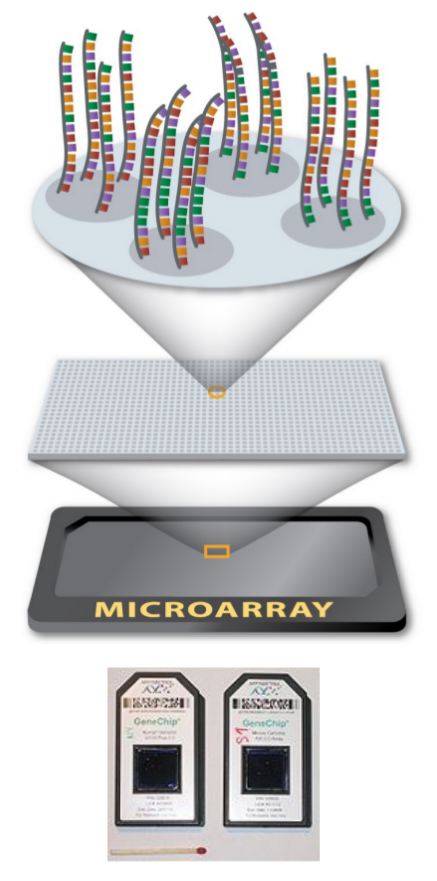
\includegraphics[scale=0.2]{microarray.png}
			\caption{Structure of a microarray}
			\label{fig:microarray}
			\end{figure}

	Moreover microarrays can have different numbers of channels:

	\begin{multicols}{2}
		\begin{itemize}
			\item $2$ channels: test and control samples are labeled with different fluorophores.
				It is a comparative technique implemented at the experiment stage of the analysis.
				After hybridization to the microarray the two samples have different colours, for example red for cancer and green for normal cells), which will be be read by a reading system.
			\item $1$ channel: one sample is loaded per time.
		\end{itemize}
	\end{multicols}

	Depending on the technology microarrays can capture, for example:

	\begin{multicols}{3}
		\begin{itemize}
			\item Exons.
			\item Genes.
			\item $3'$-ends.
		\end{itemize}
	\end{multicols}

	\subsection{Reading signal}
	A "scanner" allows to read the fluorescence light emitted by the fluorophores.
	The information is stored in $2$ images for channels arrays at $16$ bit resolution.
	The image in grey scale is represented in a red-green scale that represents the light emitted by the two fluorophores (figure \ref{fig:scanner}).

	\begin{figure}[H]
			\centering
			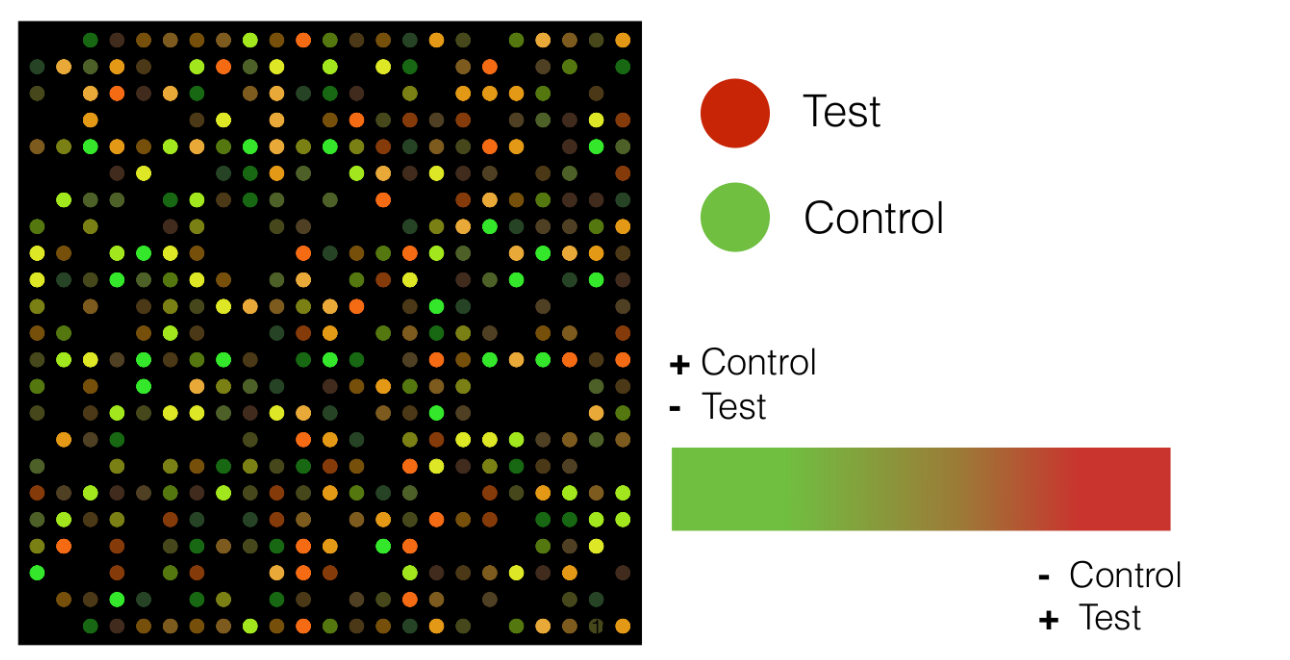
\includegraphics[scale=0.2]{scanner.png}
			\caption{The image is in grey scale but is usually represented in a red/green scale that represents the light emitted by the two fluorophores}
			\label{fig:scanner}
			\end{figure}

	If each of the spot contains probes from both samples, the resulting color will be the combination of the quantity of DNA from the two conditions that hybridized in that specific spot.
	So, the resulting color in each spot will be proportional to the quantity of test and control DNA.

	\subsection{Image analysis}
	After having obtained the images, these have to be analysed.
	This is performed by a specific technology like Affymetrix.
	The first step, after position the images on a grid, is a \textbf{segmentation} analysis: the shape and patterns inside the data is analysed to assess the signal quality for each spot (figure \ref{fig:seg}).

	\begin{figure}
	\centering
	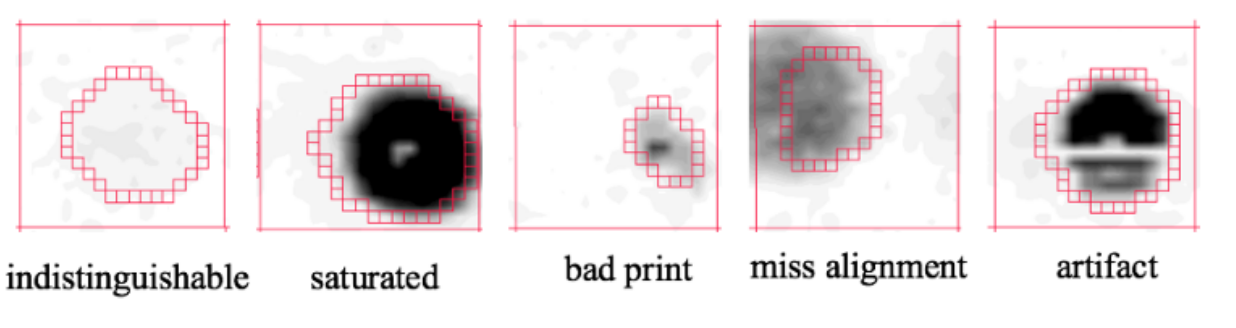
\includegraphics[scale=0.3]{segmentation}
	\caption{Result of segmentation and analysis of the result}
	\label{fig:seg}
\end{figure}


	If the quality assessed by the segmentation is fine, the analysis of the flourescent signal is performed.
	The background and foreground are identified to correct for noise generated by the former to better determine the actual data signal.
	One of the standard method for signal correction is to create a \textbf{signal model} and fit the data to it in order to evaluate the quality of the spot, for example computing the interquartile range (IQR) on the distribution in order to find feature, exclusion zone and background.
	Finally, each microarray is provided with a specific design file.
	After signal correction, the fluorescence of each spot is estimated and the relative expression for each gene (spots can be viewed as genes or portion of the genome) is interpreted thanks to annotation information.

	\begin{figure}
	\centering
	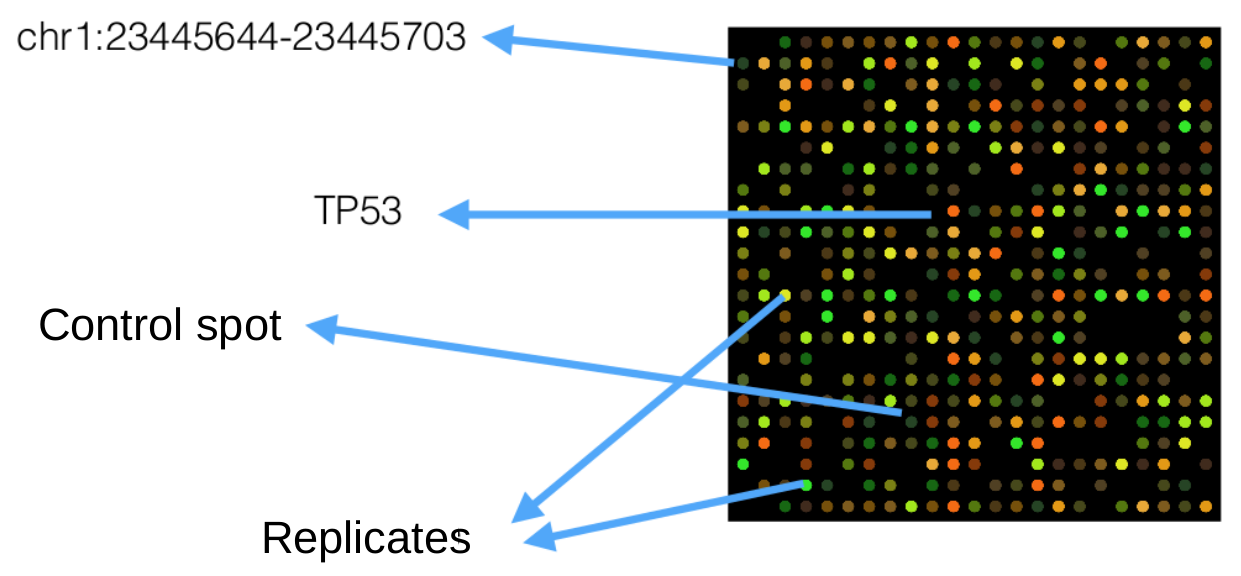
\includegraphics[scale=0.2]{design}
	\caption{Image analysis: each microarray is provided with a specific
design file}
	\label{fig:design}
\end{figure}

	For microarrays is complex to compare different technologies (but also different machines) as different probes and methods are used.
	It is always preferable to avoid performing an integrative analysis.

	\subsection{Expression microarrays}
	There are different types of arrays, but in any category, for example expression microarrays, there have sub-categories like for example, exon, gene or 3' array.
	Collecting all the signal coming from the different pieces or genes in different conditions,the quantity representing a transcript is identified for each condition, allowing to know if one condition will generate a differential expression of the gene.
	The results of micorarrays' experiments are extremely specific, making it difficult to integrate different analysis.

	\subsection{Data pre-processing}
	After the experiment is done, data pre-processing is needed to reduce errors introduced during the experimental process.
	It consists typically of:

		\begin{itemize}
			\item Background subtraction: eliminates background noise.
			\item Normalization (intra/inter sample): all samples are brought into a similar range of distribution, to reduce the effect of:

				\begin{itemize}
					\item Unequal quantity of starting sample.
					\item Differences in labeling efficiency.
					\item Differences in detection efficiency.
					\item System biases.
				\end{itemize}

			\item Summarization: aggregation of information from several spots into a single measure for each gene.
			\item Statistical quality control: removes low quality samples and probe sets.

		\end{itemize}


		\subsubsection{Two channels array}
		The pre-processing pipeline for $2$ channels array consists of different steps.

			\paragraph{Background correction}
			During background correction signal $R_s$ and $G_s$ and background estimates $R_b$ and $G_b$ are separated.
			Then the background corrected estimates $R_c$ and $G_c$ are computed as:

			$$R_c = R_s-R_b\qquad\land\qquad G_c = R_s-R_b$$

			Or as:

			$$R_c = \max(R_s-R_b, 0)\qquad\land\qquad G_c = \max(G_s-G_b, 0)$$

			\paragraph{Summarization and transforms}
			Log-ratios estimates relative expression as:

			$$\log\frac{R_c}{G_c}$$

			\paragraph{MA normalization}
			MA normalization is useful to identify systematic intensity dependent biases in the data.
			MA normalization follows empirical observations known to be present in most microarray technologies.
			The ratio of signal might depend on the average signal intensity measured across different channels, normalization gets rid of this bias.
			The function of dependence can be fitted to a polynomial regression like Loess to obtain normalization to make the plot more informative.

			$$Loess: y = f (A) \,\,\,\,\, M' = M - y$$

			\begin{figure}
			\centering
			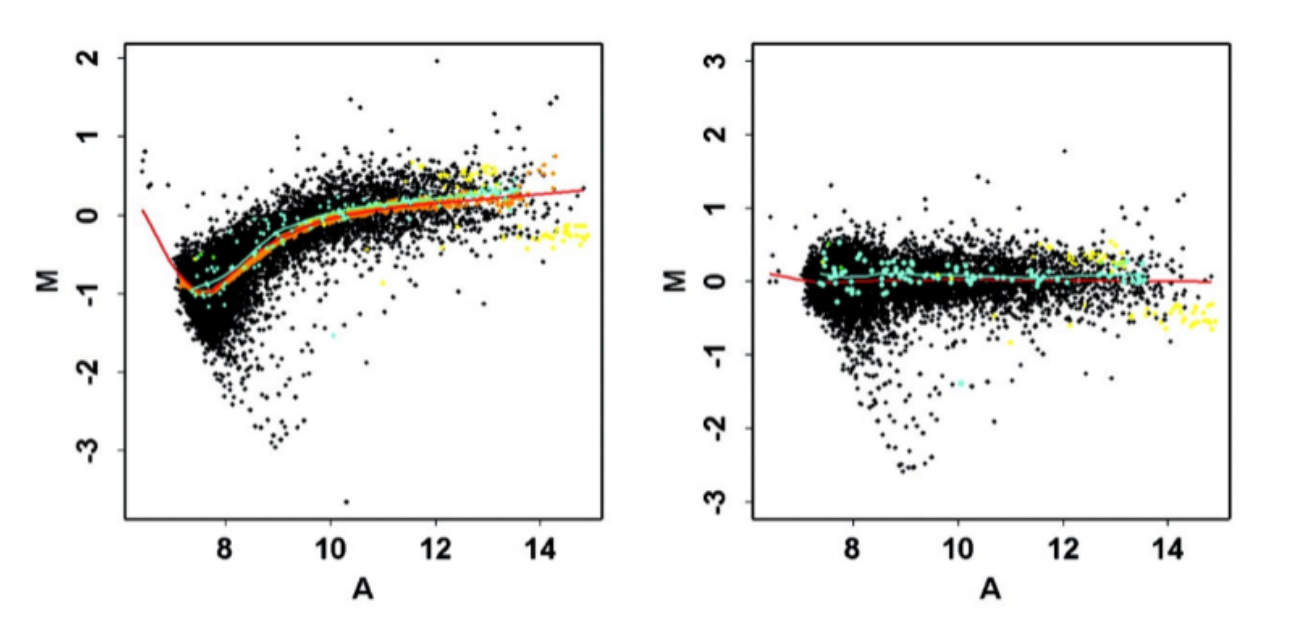
\includegraphics[scale=0.25]{MA}
			\caption{For the majority of probes, M should be equal to zero. On the right: LOESS normalization.}
			\end{figure}

			Expected $\hat{M}$ is $0$ among all observable intensities.
			This MA methodology is also very informative since it allows for performing basic DEG analysis.

		\subsubsection{One channel array}
		Many methods have been developed to pre-process Affymetrix one channel arrays:

		\begin{multicols}{3}
			\begin{itemize}
				\item Advanced methods: GCRMA, PLIER.
				\item Popular methods: RMA (discussed below) and MAS5.
				\item Rudimentary methods: MAS4, LOESS.
			\end{itemize}
		\end{multicols}

		\subsubsection{Robust Multi-array average}
		Robust multi array average is a pre-processing method that consists of three steps.

			\paragraph{Background correction}
			Background correction removes local artifacts and noise.
			The probe measure data is assumed as a combination of background noise in a normal distribution and signal in an exponential distribution.

			$$PM = Signal + Background \rightarrow Signal: S \sim e^\lambda \land Background : B\sim N(\mu, \sigma^2)$$


			By assuming strictly positive distribution of signal background, the corrected signal is also positively distributed.
			Background correction is performed on each array separately.
			$\mu$, $\sigma$ and $\lambda$ are estimated separately in each chip using the observed distributions of PMS.
			Introducing these parameters in the formula above, an estimate $E(S|PM)$ for each $PM$ value can be obtained.

			\paragraph{Normalization}
			Normalization is used to remove array effects, making all distributions the same.
			Quantile normalization is used to correct for array biases, as it compares the expression levels between arrays for various quantiles.
			It protects against outliers.
			Quantile normalization is widely used in many "inter-sample" normalization tasks.

			\paragraph{Summarization}
			Summarization combines probe intensities across arrays to get a single intensity value tor each gene or probeset.
			In median polishing each chip is normalized to its median and each gene normalized to its median.
			The procedure is repeated until medians converge.
			A maximum of $5$ iteration is allowed to prevent infinite loops.

	\subsection{Gene expression microarray}
	After pre-processing, the downstream analysis can take place, as the previous steps pre-process a trustful matrix.
	An expression microarray experiment is used to test differences in gene expression between two or more conditions, that could be for example cancer versus normal or different treatments.
	Each condition can be represented by one or more samples.
	The null hypothesis to test is that \textit{there exists no difference between the gene expression in the two conditions}.
	The comparison between the samples is done using the ratio between the test and the control samples.
	The ratio should not differ in case of null hypothesis validity.
	These ratios are also defined as \textit{fold changes}:

	$$FC = \begin{cases}Ratio & Ratio>1\\-\frac{1}{Ratio} & Ratio <1\end{cases}$$

	Fold change, at a gene level, is a ratio that represents how much the quantity of a gene changes in different conditions.
	Because ratios are not symmetric with respect to $1$ the statistics are not easy to analyze, so the log-ratio is often used.
	The log ratio of the null hypothesis should be $0$.

	$$Ratio = [0, inf] \,\, \rightarrow \,\, Log(Ratio) = [-inf, inf]$$

		\subsubsection{Replicates}
		The fold change and the log-ratio are measures that give an immediate idea of what is the difference in expression at gene level.
		It can be extended to the level of the entire gene expression profile.
		However, random deviations from the null hypothesis can happen, which can lead to the introduction of errors introducing false positives or negatives.
		To improve statistical confidence in the results, we should have replicates.
		Replicates are needed considering the noise of microarray data.
		They can be distinguished between:

		\begin{multicols}{2}
			\begin{itemize}
				\item Technical replicates: experiments on more RNA samples obtained from the \textbf{same} biological source.
				\item Biological replicates: experiments on \textbf{more} biological sources belonging to the same condition.
			\end{itemize}
		\end{multicols}

		Ideally each condition should be represented by more biological replicates, in order to perform a statistical test.
		They can also be summarized as mean for each gene.
		Ideally a matrix containing many instances for each condition should be obtained.

		\subsubsection{Statistical tests}
		Many tools for statistical analyses have been developed, which need to take into consideration, among the other parameters, noise, several replicates, thousands of genes and the multiple hypothesis problem.
		Microarray correlation can be exploited to identify differentially expressed genes.
		A gene is called differentially expressed through a $Z$ statistics.
		To find significantly differentially expressed genes a test statistic for each gene should be used.
		A low $p$-value is interpreted as evidence that the null hypothesis can be false and so a gene is differentially expressed.
		At single-gene level, basic statistics, like the T-test can be applied.

			\paragraph{T-Test}

			The T-test is a parametric test to check the difference between the mean of two groups.
			It assumes that the variance of those two groups is the same.
			Is computed as:

			$$T(X, Y) = \frac{\bar{X}-\bar{Y}}{\sigma\sqrt{\frac{1}{m}+\frac{1}{n}}}$$

			\paragraph{Walch t-test}
			Walch t-test considers different variance between two groups, an extension of t-test.
			It is the default implementation for $R$ $t.test()$ function.
			Is computed as:

			$$T(X, Y) = \frac{\bar{X}-\bar{Y}}{\sqrt{\frac{\sigma^2_{X}}{m}+\frac{\sigma^2_Y}{n}}}$$

			\paragraph{Wilcoxon test}
			The Wilcoxon test is a non parametric test to check the equality of two distributions.

			\paragraph{Permutation test}
			The permutation test generates a null distribution on an observation of interest by changing the group labels.
			It compares the values observed in data and the values in the generated null distribution.
			Is computed as:

			$$p = \frac{\#\{b:|T_b|\ge T_{obs}\}}{B}$$

		\subsubsection{Correction methods}
		Correction methods are used to correct p-values in the presence of \textbf{multiple null hypothesis}.
		Correction for this problem is extremely important.
		Say we have a set of hypothesis we want to test simultaneously, like for a microarray setting.
		Considering $n$ multiple hypothesis the probability of observing one significant result due to chance is:

		$$1-(1-pvalue)^n$$

		Some examples of correction methods are:

		\begin{multicols}{2}
			\begin{itemize}
				\item Bonferroni: very conservative, it has a significance threshold of $\frac{\alpha}{N}$.
					It reduces false positive while introducing false negatives.
				\item Benjamini-Hochenberg: it tunes false positives and false negatives.
				\item False Discovery Rates: it checks if the $kth$ ordered p-value is larger than $\frac{k\cdot a}{N}$
			\end{itemize}
		\end{multicols}

		\paragraph{ANOVA analysis}
			ANOVA analysis is a method for multiple hypothesis analysis and is used to control different treatments.
			It allows to test the null hypothesis that the differences within and between at least $3$ groups are the same on average.

			\paragraph{2-way ANOVA}
			2-way ANOVA is another multiple null hypothesis analysis method: it compares the mean differences between groups that have been split on two independent variables called factors.
			It understand if there is an interaction between the two independent variables on the dependent one.


		\subsubsection{Receiver Operating Characteristic}
		At the end, of the analysis of gene expression data a ROC curve is generated.
		The receiver Operating Characteristic finds genes that better discriminate between two conditions by plotting sensitivity and $1-$specificity.
		Let $AUC$ be the area under the $ROC$ curve, then:

		\begin{multicols}{2}
			\begin{itemize}
				\item $AUC=1$: perfect classification.
				\item $AUC = 0.5$: random classification.
			\end{itemize}
		\end{multicols}

		\begin{figure}
	\centering
	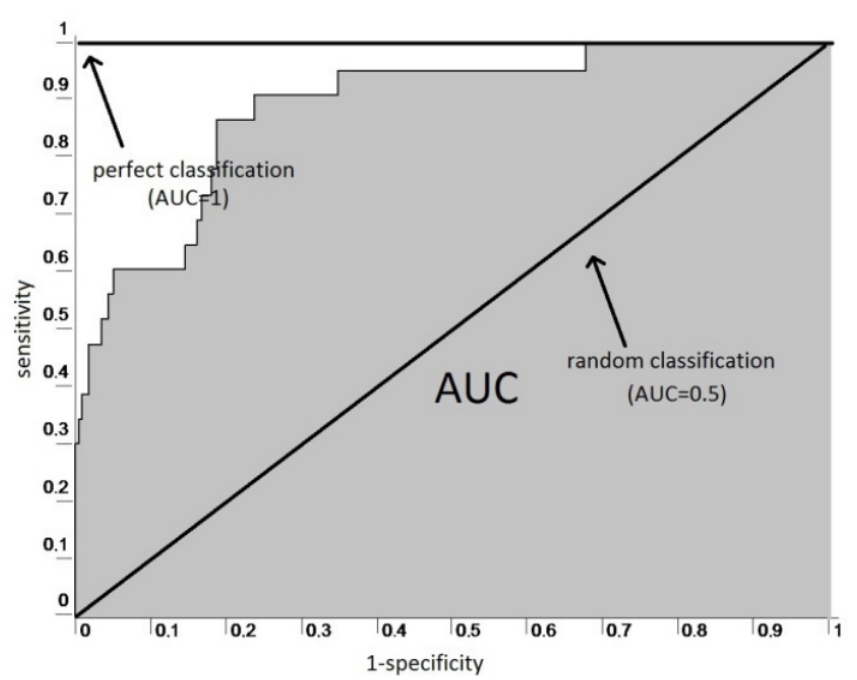
\includegraphics[scale=0.2]{ROC}
	\caption{Allows to find genes that better discriminate between the two conditions}
	\label{fig:design}
\end{figure}

		\subsubsection{Clustering}
		The objective in differential gene expression is to look for genes that behave differently between samples, either up- or down- regulated.
		In clustering, the deregulated genes are aggregated together, to see if they form some patterns, maybe they come from the same pathways which is overall deregulated.
		Once having obtained then they can be clustered according to similar expression to make the outliers more obvious.

			\paragraph{Hierarchical clustering}
			The algorithm creates a dendrogram based on on the definition of a distance (dissimilarity) measure between observation pairs.
			The algorithm works as follows:

				\begin{itemize}
					\item Starting with $N$ observations and a distance measure like euclidean distance or Pearson correlation factor for all $\frac{N(N-1)}{2}$ pairs.
						At the beginning, each observation is a cluster.
					\item For $i =n$ to $2$:

						\begin{itemize}
							\item Examine all inter-clusters distances and fuse the cluster with lower distance.
								The distance between fused clusters represents the height of the bar in the dendrogram.
							\item Calculate new inter-cluster distances between the remaining $i-1$ clusters.
						\end{itemize}

				\end{itemize}

			\paragraph{Linkage}
			Linkage defines the distance between clusters (containing many observations), as the distance measure is only used between single samples (clusters with one instance).

			\begin{figure}
	\centering
	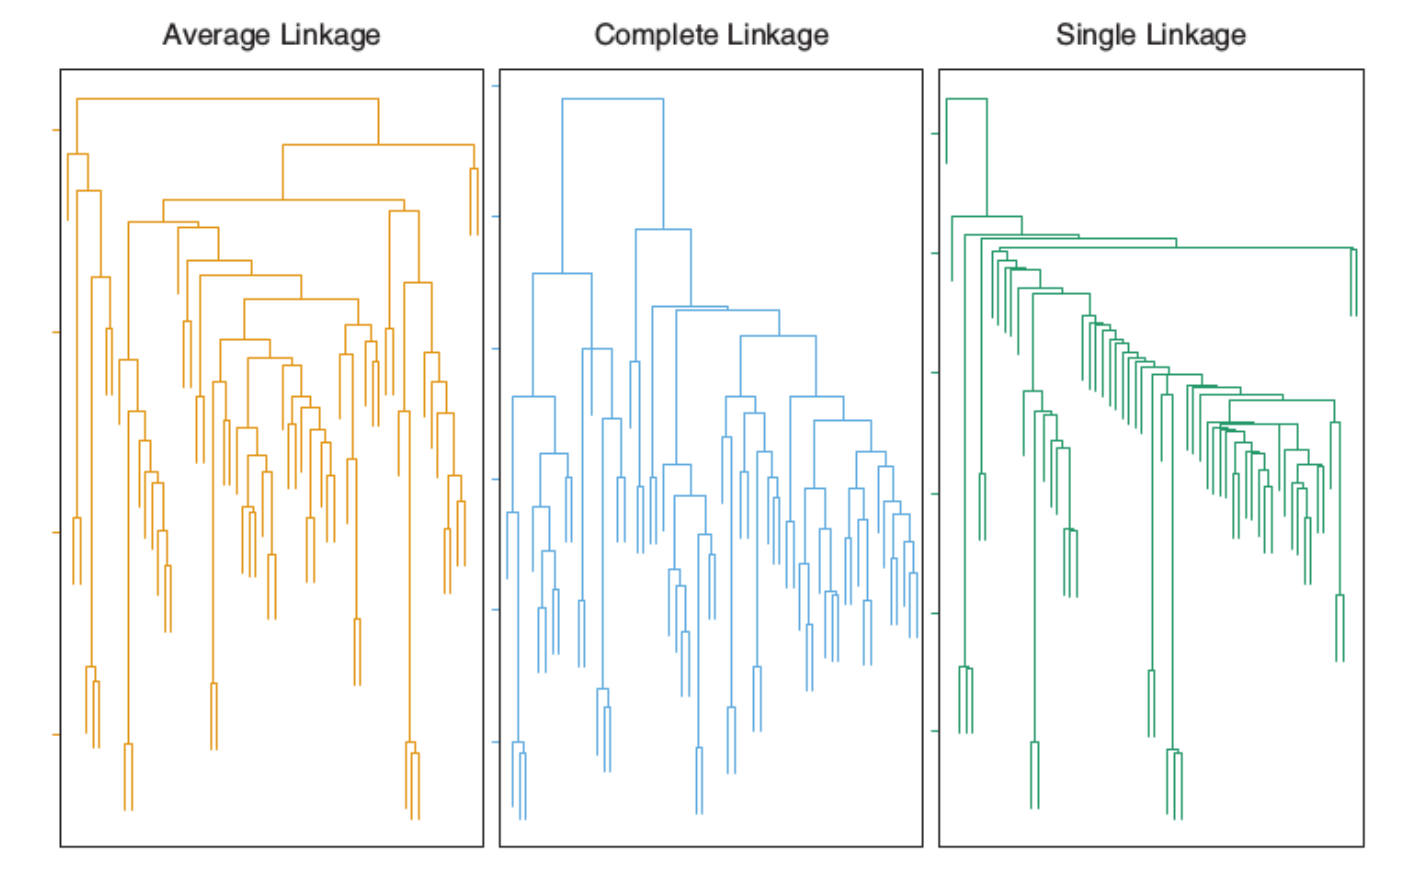
\includegraphics[scale=0.2]{linkage}
	\caption{Different linkage methods. The length of the branches represents the distance between samples.}
	\label{fig:linkage}
\end{figure}

				\subparagraph{Complete linkage}
				In complete linkage maximal intercluster dissimilarity is reached.
				Computes all pairwise dissimilarities between the observations in cluster $A$ and in cluster $B$, and record the \textbf{largest} of these dissimilarities.

				\subparagraph{Single linkage}
				In single linkage minimal interclsuter dissimilarity is reached.
				All pairwise dissimilarities between the observations in cluster $A$ and in cluster $B$ are computed and the \textbf{smallest} is recorded.
				It can result in extended, trailing clusters in which single observations are fused one at a time.

				\subparagraph{Average linkage}
				In average linkage te mean intercluster dissimilarity  is reached.
				All pairwise dissimilarities between the observations in cluster $A$ and in cluster $B$ are computed and the \textbf{average} is recorded.

				\subparagraph{Centroid linkage}
				In centroid linkage the dissimilarity between the centroid for cluster $A$ (a mean vector of length $p$) and for cluster $B$ is computed and recorded.
				It can result in undesirable \textbf{inversions}.


\section{RNA-sequencing}
	RNA sequencing is a next-generation sequencing approach that sequences the cDNA from the mRNA component.
	RNA-seq is considered a high-throughput technology because the whole transcriptome can be sequenced in one shot.
	The whole transcriptome can be compared against the whole transcriptome of another sample.
	It is very cheap, sequencing $\sim 400$ gigabases per flow cell, but it has an error rate up to $1\%$, issues with $AT$ and $GC$ regions and long sequencing items.

	\subsection{Issues}
	RNA-seq shares some litigations with microarray technology.
	For example, one needs availability of biological replicates (at least $3$) and to take care of batch effects to derive confident conclusions.
	RNA-seq also requires the selection of a sequencing protocol after library preparation.
	For example, the choice of PE over SE, controlling the read length (100/150 bp) and sequencing depth (20-50M per sample for differential expression).

	\subsection{Illumina's protocol}
	Illumina's RNA-sequencing pipeline consists of different steps.

		\subsubsection{Sample preparation}
		In sample preparation RNA is extracted and sheared into $300$-$600np$ fragments through sonication or enzymatic digestion.

		\subsubsection{Library preparation}
		During library preparation adapter sequences are ligated to the fragments.
		Barcoding is possible allowing for sample multiplexing.

		\subsubsection{Cluster generation}
		During cluster generation the library is amplified through PCR and loaded into a flow cell where fragments are captured on a lawn of surface-bound oligos complementary to the library adapters.

		\subsubsection{Sequencing}
		Sequencing is done by synthesis: sequencing reagents, including fluorescently labelled nucleotides are added and the first base is incorporated.
		The flow cell is imaged and the emission from each cluster is recorded.
		The emission wavelength and intensity are used to identify the base.
		This cycle is repeated $n$ times to create a read length of $n$ bases.

		\begin{multicols}{2}
			\begin{itemize}
				\item Paired ends are used for duplicates, splicing analysis and discovery of novel isoforms.
				\item Single ends are used for gene expression analysis.
			\end{itemize}
		\end{multicols}

		\subsubsection{Alignment}
		Reads, stored in a FASTQ file, are aligned to a reference genome or transcriptome or to a genomic region.
		\textbf{Splice-aware} aligner such as TopHat or STAR should be used.
		The alignments are refined according to coding sequences using known and predicted splice junctions.
		Splice-aware alignment is nowadays pretty fast, it is implemented though heuristic methods which converges to satisfying results.
		Alternatively, reads can be assembled de novo through a tool like Trinity.

		\subsubsection{Quantifying reads per gene}
		The aim of read quantification is to count sequence reads per gene (parallel to quantify the fluorescence signal in microarray).
		Several decision and precautions must be made when mapping reads to the genome.
		For example filtering out rRNA, tRNA and mitRNA is necessary, while non-coding RNA can be included or excluded depending on the type of analysis performed.
		Alternative splicing, overlapping genes and pseudogenes are dealt with.
		Moreover, different type of counts can be employed:

			\paragraph{Counts used by differential expression methods}
			Counts used for differential expression analysis are:

			\begin{itemize}
				\item \textbf{Standard count}: number of reads for transcript.
				\item \textbf{CPM}: counts scaled by the number of fragments sequenced $N$ times one million.
					It allows to compare each transcript across different samples.

					$$CPM_i = \frac{X+i}{N}\cdot 10^6$$

				\item \textbf{RPKM}: reads per kilobase of exon per million reads mapped.
					It is called FPKM for fragments.
					It's the most common type of count used.


					$$RPKM = \frac{X_i}{\big(\frac{\tilde{l}_i}{10^3}\big)\big(\frac{N}{10^6}\big)} = \frac{X_i}{\tilde{l}_iN}10^9$$

					The typical length of a gene and the typical number of reads generated by a RNA-seq experiments are taken into account by the constants.
			\end{itemize}

			\paragraph{Intra-sample normalization}
			The most common count used for intra-sample normalization is \textbf{TPM}
			It is the measurement of the proportion of transcripts in the pool of RNA.
			It takes into account the length of the transcript, more reads that fall into that gene.
			Let $\tilde{l}_i$ the length of transcript $i$, then:

			$$TPM_i = \frac{X_i}{\tilde{l}_i}\biggl(\frac{1}{\sum\limits_j\frac{X_j}{\tilde{l}_j}}\biggr)10^6$$

		\subsubsection{Inter sample normalization}
		To perform inter-sample normalization quantile normalization is used to make the distribution identical.
		The best normalization methods for differential expression are coupled with sophisticated approaches as very low expressing genes are tricky, for example those with $FPKM<1$.
